%------------------------------------------------------------------------
%Editar Diplomado
\hypertarget{cv:registrarColaborador}{\section{Registrar Colaborador}} \label{sec:registrarColaborador}

	Esta funcionalidad le permitirá registrar un colaborador que podrá participar dentro de un proyecto ya sea como analista o como líder. 

		\subsection{Procedimiento}

			%Pasos de procedimiento
			\begin{enumerate}
	
			\item Oprima el botón \IURegistrar{} de la pantalla \ref{fig:GestionarColaboradores} ''Gestionar Colaboradores''.
			
			\item Se mostrará la pantalla \ref{fig:registrarColaborador} ''Registrar Colaborador''.

			%Pantalla
			\begin{figure}[htbp!]
				\begin{center}
					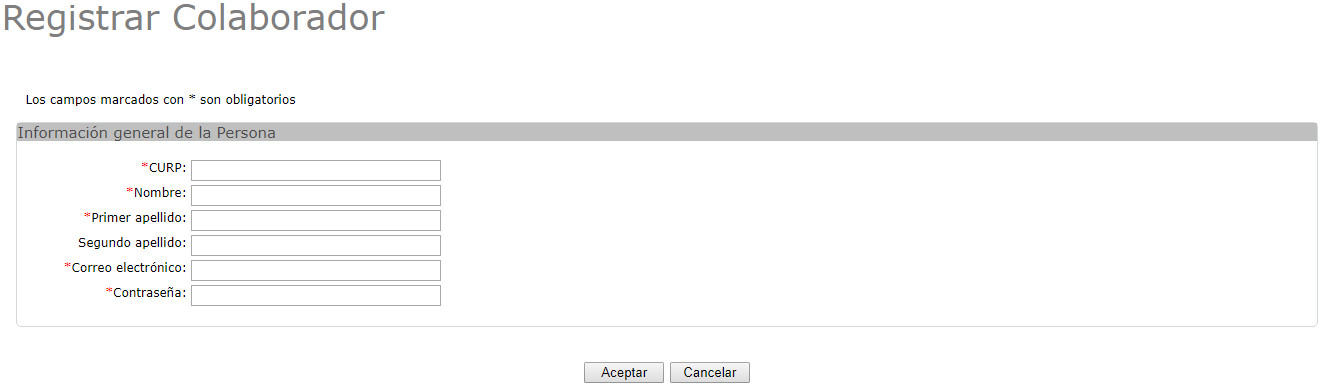
\includegraphics[scale=0.6]{roles/administrador/colaboradores/gestionarColaboradores/pantallas/IU3-1registrarPersona}
					\caption{Registrar Colaborador}
					\label{fig:registrarColaborador}
				\end{center}
			\end{figure}
		
			\item Ingrese la CURP, nombre y apellidos del colaborador. Posteriormente ingrese el correo electrónico y la contraseña las cuales servirán como credenciales para ingresar a TESSERACT.
			
			\item Oprima el botón \IUAceptar.
			
			\item Se mostrará el mensaje \ref{fig:colaboradorRegistrado} en la pantalla \ref{fig:registrarColaborador} ''Gestionar Colaboradores''.
			
			\begin{figure}[htbp!]
				\begin{center}
					
\includegraphics[scale=0.6]{roles/administrador/colaboradores/gestionarColaboradores/pantallas/IU3-1MSG1}
					\caption{MSG: Colaborador Registrado}
					\label{fig:colaboradorRegistrado}
				\end{center}
			\end{figure}
			\end{enumerate}